\chapter{증명법}

1장에서 얘기한 것 처럼 모든 수학 문제는 \textbf{명제}이고, 수학 문제를 푸는 것은 명제가 참이 되도록 가정 또는 결론을 채우는 것이다. 그런데 수학에서 어떤 명제가 참이라고 주장하기 위해서는 \textbf{논리적인 과정을 통해 그 명제가 참임을 증명}해야 한다. 사실상 \textbf{풀이 과정이 곧 증명}인 셈이다.

수학 공부를 하다 보면 개념을 공부할 때 어떤 정리나 성질에 대한 증명을 접하기도 하고, 서술형 문제를 만나 풀이 과정(증명)을 적기도 하고, 나아가 명시적으로 어떤 사실을 증명하라는 문제를 접하기도 한다.

한편, 이러한 증명들은 학교 시험에 잘 출제되지 않는 편이며, 일반적으로 서술형 문제의 비중은 객관식 문제에 비해 낮은 편이다. 나아가 이와 같은 문제들은 모의고사나 수능에 아예 출제되지도 않는다. 그러다 보니 많은 학생들이 증명의 중요성을 간과하게 된다.

수학 공부에서 증명이 중요한 이유는 간단하다. \textbf{증명을 적으며 수학적으로 성장}하기 때문이다. 증명을 적는 과정은 \textbf{배운 것을 올바르게 정리하는 과정}이다. 그러므로 증명에 사용된 개념을 더욱 명확하게 이해하게 되고, 증명이 논리적으로 올바른지 스스로 판단하는 \textbf{수학적 사고력}을 기르게 된다.

또한 증명은 \textbf{개념에 대한 깊이있는 이해}를 돕는다. 증명 속에 숨겨진 아이디어를 배우게 되고, 증명을 이해하면 해당 명제의 진정한 의미를 이해하게 되기도 한다. 이렇게 얻은 수학적 사고방식과 개념에 대한 이해는 \textbf{고난도 문제를 해결하는 강력한 도구}가 되어, 기계적인 문제 풀이와는 차원이 다른 성장을 가져다 준다.

그러나 증명을 적는 것은 결코 쉽지 않기 때문에 많은 시간과 훈련이 필요하다. 2\(\sim\)3장에서 배운 내용을 바탕으로 논리적 추론 규칙을 이용한 단계적인 사고에 익숙해지고, 모든 문제의 풀이를 증명하듯 차근차근 적다 보면 어느새 증명에 익숙해진 성장한 자신을 발견하게 될 것이다.

이번 장에서는 참인 명제를 증명하는 3가지 대표적인 방법과, 명제가 거짓임을 증명하기 위해 반례를 찾는 방법을 소개한다.

\section{직접증명법}

직접증명법은 말 그대로 주어진 명제를 직접 증명하는 방법이다. \(p \ra q\) 형태의 명제가 주어지면, 가정 \(p\)에서 시작해 논리적인 과정을 거쳐 \(q\)에 도달하게 되며, 그 과정에서 배운 내용을 총 동원하게 된다.

결국 증명 또한 일종의 문제 해결 과정이기 때문에, 앞서 설명한 내용이 그대로 적용된다.
\begin{enumerate}
    \item 주어진 것과 구하는 것을 파악한다.
    \item \textbf{주어진 것과 구하는 것을 바탕으로} 배운 명제 중 적용할 수 있는 것이 있는지 찾아본다.
    \item \textbf{논리적 추론 규칙을 사용한다.}
\end{enumerate}

다음 예제를 통해 알아보자.

\begin{wrapfigure}{R}{0.36\textwidth}
    \begin{tikzpicture}[scale=1.2]
        \coordinate (A) at (0, 0);
        \coordinate (B) at (4, 0);
        \coordinate (P) at (2, 1.959);
        \coordinate (Q) at (2, -1.959);

        \draw[-, very thick] node[below left] {\(\rm{A}\)} (A) -- (B) node[below right] {\(\rm{B}\)};

        \draw[red] ([shift=(-53:2.8)] A) arc (-53:53:2.8);
        \draw[red] ([shift=(127:2.8)] B) arc (127:233:2.8);

        \draw[dotted, very thick] (2, 2.3) -- (2, -2.3);

        \filldraw[fill=black] (A) circle (0.03);
        \filldraw[fill=black] (B) circle (0.03);
        \filldraw[fill=black] (P) circle (0.03) node[right=2] {\(\rm{P}\)};
        \filldraw[fill=black] (Q) circle (0.03) node[right=2] {\(\rm{Q}\)};
    \end{tikzpicture}
    \vspace{-50px} % workaround...
\end{wrapfigure}

\bigskip

\ex. (수직 이등분선의 작도)

다음은 \(\linesegment{AB}\)의 수직 이등분선 \(\linesegment{PQ}\)를 작도하는 방법이다.
\begin{enumerate}
    \item \(\linesegment{AB}\)의 길이 절반보다 길게 컴퍼스를 벌린다.
    \item \(\rm{A}\)와 \(\rm{B}\)를 각각 중심으로 원의 일부(호)를 그린다.
    \item 그린 호의 두 교점을 각각 \(\rm{P}\), \(\rm{Q}\)라 하자.
    \item 자로 \(\linesegment{PQ}\)를 그린다.
\end{enumerate}

\bigskip

위와 같이 작도한 \(\linesegment{PQ}\)가 \(\linesegment{AB}\)를 수직 이등분함을 증명하여라.

\newpage

문제를 차근차근 파악해 보자. \textbf{우선 주어진 것과 구하는 것은 무엇인가?} 작도 과정이 주어진 것은 알겠는데, 이로부터 정보를 얻어내야 한다. 문제를 풀 때 주어진 것으로부터 조건을 끄집어낸 경험을 많이 해봤을 것이다.

우선 (1)은 컴퍼스를 조절하는 과정이니 넘어간다.\footnote{왜 \(\linesegment{AB}\)의 길이 절반보다 길게 벌리라고 했을까?} 작도 과정 (2), (3)을 보면 두 점을 중심으로 \textbf{원}의 일부를 두 개 그렸고, 그 교점을 잡았다. 원의 \textbf{정의}가 무엇인가? 중심이라는 한 점으로부터 거리가 같은 점들의 모임이다. 그러므로 다음 사실을 알 수 있다.
\begin{center}
    \(\linesegment{AP} = \linesegment{AQ} = \linesegment{BP} = \linesegment{BQ}\)
\end{center}
(4)는 두 교점을 연결한 것이므로 특별히 얻어낼 정보는 없어 보인다. 만약 원의 정의를 제대로 알고 있지 않았다면, 위와 같은 사실을 얻어내지 못해 문제 풀이를 시작조차 하지 못했을 것이다.

다음으로 구하는 것을 파악해야 한다. 구하는 것은 \(\linesegment{PQ}\)가 \(\linesegment{AB}\)의 \textbf{수직 이등분선}인 것에 대한 증명이다. 수직 이등분선의 \textbf{정의}가 무엇인가? 선분과 수직으로 만나면서 선분을 이등분하는 직선이다. 따라서 \(\linesegment{PQ}\)와 \(\linesegment{AB}\)가 수직으로 만나고, 그 교점이 \(\linesegment{AB}\)의 중점이 된다는 사실을 모두 증명해야 한다. 증명의 편의상 교점을 \(\rm{M}\)이라 두면, 구하는 것은 다음과 같다.
\begin{center}
    \(\angle \rm{AMP} = 90^\circ\) 이고 \(\linesegment{AM} = \linesegment{BM}\).\footnote{각의 경우 꼭 \(\angle \rm{AMP}\)일 필요는 없다. 네 각 중 어느 것을 골라도 된다. 왜 그런가?}
\end{center}
마찬가지로 수직 이등분선의 정의를 제대로 알고 있지 않았다면, 구하는 것이 무엇인지도 모른 채 문제를 풀지 못하고 헤매게 되었을 것이다.

문제 파악이 완료되었다. 이 문제의 핵심만 간추려 명제로 요약하면 다음과 같다.
\begin{center}
    \(\linesegment{AP} = \linesegment{AQ} = \linesegment{BP} = \linesegment{BQ}\) 일 때, \(\angle \rm{AMP} = 90^\circ\) 이고 \(\linesegment{AM} = \linesegment{BM}\) 이다.
\end{center}
\textbf{이제 적용할 수 있는 명제가 있는지 가정과 결론을 바탕으로 생각해야 한다.} 가정과 결론을 다시 보니 선분의 길이가 같다는 내용이 많이 포함되어 있다. 길이가 같다는 내용을 어디서 배웠더라?

바로 \textbf{도형의 합동}이다! 두 도형이 합동이면 대응변의 길이와 대응각의 크기가 같다는 사실을 배웠다.\footnote{중학교 1학년의 지식만 이용한다면 사실상 이 방법 밖에 없다고 봐야할 것이다.} 이 사실의 결론은 우리가 구하고자 하는 결론 \(\linesegment{AM} = \linesegment{BM}\) 에 들어맞는다. 추가로, 자연스럽게 \(\angle \rm{AMP} = 90^\circ = \angle \rm{BMP}\) 도 생각하게 된다. 그렇다면 \(\linesegment{AM}\)과 \(\linesegment{BM}\)을 대응변으로, \(\angle \rm{AMP}\)와 \(\angle \rm{BMP}\)를 대응각으로 포함하는 서로 다른 두 도형을 생각하고, 두 도형이 합동임을 보여야 한다.

두 도형이 합동인 것은 어떻게 알더라? 분명 합동을 공부하면서 \textbf{합동 조건}을 배웠었다. 삼각형의 경우 SSS, SAS, ASA 합동 조건이 있으며, 원의 경우 반지름이 같으면 합동이고, 정다각형의 경우 한 변의 길이만 같아도 합동이 된다는 사실을 배웠다.

그림을 잠깐 다시 보니, 현재 우리의 상황에 가장 적합한 접근 방향은 \textbf{삼각형의 합동 조건}을 이용하는 것이라 생각할 수 있다. 합동임을 보이려는 도형이 \(\linesegment{AM}\)과 \(\linesegment{BM}\)을 포함해야 하는데, 이 선분은 원의 일부가 아니며, 문제에는 정다각형에 대한 언급이 어디에도 없다. 따라서 삼각형의 합동 조건이 문제를 해결하는 열쇠가 될지 아직은 모르더라도, \textbf{주어진 것과 구하는 것을 바탕으로 생각했을 때 문제를 해결할 가능성이 가장 높은 방향이라 판단할 수 있다}.

\begin{wrapfigure}{R}{0.36\textwidth}
    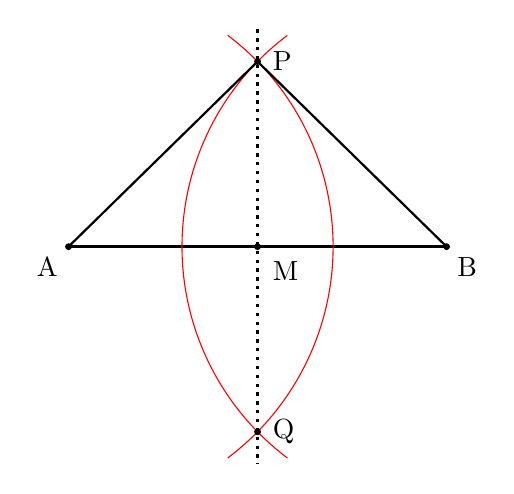
\begin{tikzpicture}[scale=1.2]
        \coordinate (A) at (0, 0);
        \coordinate (B) at (4, 0);
        \coordinate (P) at (2, 1.959);
        \coordinate (Q) at (2, -1.959);
        \coordinate (M) at (2, 0);

        \draw[-, very thick] node[below left] {\(\rm{A}\)} (A) -- (B) node[below right] {\(\rm{B}\)};

        \draw[red] ([shift=(-53:2.8)] A) arc (-53:53:2.8);
        \draw[red] ([shift=(127:2.8)] B) arc (127:233:2.8);

        \draw[thick] (A) -- (P) -- (B);
        \draw[dotted, very thick] (2, 2.3) -- (2, -2.3);

        \filldraw[fill=black] (A) circle (0.03);
        \filldraw[fill=black] (B) circle (0.03);
        \filldraw[fill=black] (P) circle (0.03) node[right=2] {\(\rm{P}\)};
        \filldraw[fill=black] (Q) circle (0.03) node[right=2] {\(\rm{Q}\)};
        \filldraw[fill=black] (M) circle (0.03) node[below right=2] {\(\rm{M}\)};
    \end{tikzpicture}
    \vspace*{-20px}
\end{wrapfigure}

이제 \(\linesegment{AM}\)과 \(\linesegment{BM}\)을 대응변으로, \(\angle \rm{AMP}\)와 \(\angle \rm{BMP}\)를 대응각으로 포함하는 \textbf{삼각형}을 찾아보자. 여기서 한 가지 고려사항은, \textbf{최대한 알고 있는 내용을 활용할 수 있는 방향으로 찾아야 한다}는 점이다.\footnote{사실은 \(\rm{A}, \rm{B}, \rm{M}\)은 이미 삼각형에 포함되어야 하므로 제외하면, 우리에게 남은 선택지는 \(\rm{P}, \rm{Q}\) 두 개이다. 그런데 이마저도 대칭성으로 인해 사실상 우리에게 선택지는 \(\rm{P}\) 하나 뿐이므로, 자연스럽게 \(\triangle \rm{AMP}\)와 \(\triangle \rm{BMP}\)를 생각하게 된다. 하지만 복잡한 문제에서는 선택지가 많기 때문에, 알고 있는 내용을 활용할 수 있는 방향으로 찾아야 한다는 의미이다.} 우리는 \(\linesegment{AP} = \linesegment{BP}\) 를 알고 있으므로, 이를 이용할 수 있는 \(\triangle \rm{AMP}\)와 \(\triangle \rm{BMP}\)를 생각하게 된다.

그러나 당장 이 두 삼각형이 합동임을 보이기는 어려워 보인다. \(\linesegment{AP} = \linesegment{BP}\) 임을 알고, \(\linesegment{PM}\)이 공통임을 알고 있지만, 삼각형의 합동 조건을 생각하면 조건 3개가 필요하므로 하나가 부족한 상황이다.

한 번에 풀리지는 않으니, \textbf{삼단논법의 징검다리}를 사용해 보자. 현재 우리는 징검다리 명제의 결론으로 삼각형의 합동 조건을 사용하려 하고 있다. 그렇다면 징검다리 명제의 가정은 SSS, SAS, ASA 중 하나일 것이다.\footnote{예를 들어, 삼각형의 세 쌍의 대변의 길이가 모두 같으면(가정), 두 삼각형은 합동이다(결론).}

세 개 중 어느 것을 써야 할지는 마찬가지로 \textbf{주어진 것과 구하는 것을 보면} 알 수 있다. 이미 두 쌍의 대변의 길이가 같다는 사실을 알고 있고, 각에 대한 정보가 없기 때문에, ASA는 가정으로 사용할 수 없다. 또한, 마지막 한 쌍의 대변인 \(\linesegment{AM}\)과 \(\linesegment{BM}\)은 구하는 것이므로 합동임을 보인 뒤 얻게 되는 결론이기 때문에 합동 조건의 가정에 포함될 수 없다. 따라서 SSS 합동 조건도 가정 후보에서 자동으로 제외된다.

남은 것은 SAS 합동조건 뿐이고, 이를 사용하기 위해서는 두 변 사이의 끼인각 \(\angle \rm{APM}\)과 \(\angle \rm{BPM}\)이 같아야만 한다. 이 사실을 얻을 수 있을까? 이를 위해 징검다리를 하나 더 써야할 듯 하다. 마찬가지로 각이 같음을 증명해야 하기 때문에, 합동을 생각하게 되고, 위와 비슷한 논리로 삼각형의 합동을 생각하게 된다.

어떤 삼각형을 잡아야 할까? \textbf{주어진 것을 다시 보자. 아직 사용하지 않은 조건이 있다!} \(\linesegment{AP} = \linesegment{BP}\) 이기도 하지만, 이들의 길이는 \(\linesegment{AQ}\), \(\linesegment{BQ}\)와도 같다. 이를 사용하기 위해, 그리고 두 끼인각이 같음을 보이기 위해 잡아야 하는 두 삼각형으로는 \(\triangle \rm{APQ}\)와 \(\triangle \rm{BPQ}\)가 적절해 보인다. 이미 두 쌍의 대변의 길이가 같고, \(\rm{PQ}\)가 공통이므로, SSS 합동 조건에 의해 \(\triangle \rm{APQ} \equiv \triangle BPQ\) 이기 때문이다.

증명이 거의 완성되었다. \(\triangle \rm{APQ} \equiv \triangle BPQ\) 이므로, 대응각이 같아 \(\angle \rm{APM} = \angle \rm{BPM}\) 이다.\footnote{이 사실이 왜 필요했더라? \textbf{주어진 것과 구하는 것을 항상 생각}하면 가정에서 결론으로 가는 복잡한 증명길 속에서도 길을 잃지 않을 수 있다.} 따라서 SAS 합동 조건을 적용할 수 있고, \(\triangle \rm{AMP} \equiv \triangle \rm{BMP}\)를 얻는다. 합동임을 보였기 때문에 우리의 최종 결론인 \(\angle \rm{AMP} = 90^\circ\) 와 \(\linesegment{AM} = \linesegment{BM}\) 은 자동으로 얻어진다.

\bigskip

문제를 해결하는 사고방식과 사고의 흐름을 숨김 없이 밝히다 보니 풀이 과정이 매우 길어졌다. 답안으로 적기 위해 다시 흐름을 정리하면 다음 그림처럼 나타낼 수 있다.\footnote{각 단계의 화살표에서 사용된 명제나 논리적 추론 규칙이 무엇인지 확인해 보라.}
\[
    \begin{tikzcd}
        & \linesegment{AP} = \linesegment{BP} = \linesegment{AQ} = \linesegment{BQ} \arrow{ddd} \arrow{dr} &  \\
        & & \linesegment{AP} = \linesegment{BP}, \; \linesegment{AQ} = \linesegment{BQ} \arrow{d} & \linesegment{PQ}\text{는 공통} \arrow{dl} \\
        & & \triangle \rm{APQ} \equiv \triangle \rm{BPQ} \arrow{d} & \\
        \linesegment{PM}\text{은 공통} \arrow{dr} & \linesegment{AP} = \linesegment{BP} \arrow{d} & \angle \rm{APM} = \angle \rm{BPM} \arrow{dl} \\
        & \triangle \rm{AMP} \equiv \triangle \rm{BMP} \arrow{d} \arrow{dr} & & \\
        & \angle \rm{AMP} = 90^\circ = \angle \rm{BMP} & \linesegment{AM} = \linesegment{BM} &
    \end{tikzcd}
\]
이를 답안의 형태로 적으면 다음과 같다. 보통 답안에는 사고의 과정은 생략하고 필요한 내용만 적기 때문에 훨씬 짧아진다.\footnote{풀이과정이나 증명을 어떻게 쓸지 모르겠다면 해설지를 참고하는 것도 좋은 방법이다.}

\pf \(\linesegment{AB}\)와 \(\linesegment{PQ}\)의 교점을 \(\rm{M}\)이라 하자. 작도 과정의 (2), (3)단계에 의해 \(\linesegment{AP} = \linesegment{BP} = \linesegment{AQ} = \linesegment{BQ}\) 이다. 그러므로 \(\linesegment{AP} = \linesegment{BP}\), \(\linesegment{AQ} = \linesegment{BQ}\), \(\linesegment{PQ}\)는 공통이므로 SSS 합동 조건에 의해 \(\triangle \rm{APQ} \equiv \triangle \rm{BPQ}\) 이다. 이로부터 \(\angle \rm{APM} = \angle \rm{BPM}\) 임을 알 수 있다. 한편, \(\linesegment{PM}\)이 공통이고 \(\linesegment{AP} = \linesegment{BP}\) 이므로 SAS 합동 조건에 의해 \(\triangle \rm{AMP} \equiv \triangle \rm{BMP}\) 이다. 따라서 \(\linesegment{AM} = \linesegment{BM}\) 이고, \(\angle \rm{AMP} = \angle \rm{BMP}\) 인데, 두 각은 합쳐서 \(180^\circ\)이므로 각각은 \(90^\circ\)이어야만 한다. 그러므로 \(\linesegment{PQ}\)는 \(\linesegment{AB}\)를 중점 \(\rm{M}\)에서 수직 이등분한다. \qed

위 증명에 천재적인 아이디어가 들어갔다고 생각하는가? \textbf{절대 아니다!} 위 증명을 포함하여 대부분의 문제들은 \textbf{천재적인 아이디어를 요구하지 않는다.} 단지 \textbf{주어진 것과 구하는 것을 바탕으로 배운 것들을 적용하기 위해 논리적으로 생각}했을 뿐이다. 이는 여러 번 강조해도 부족하다!

해설지의 풀이를 보면 우리가 모르는 내용을 사용해서 푸는 경우는 거의 없다. 전부 배운 내용을 바탕으로 하고 있다. 이는 문제를 푸는 입장에서 배운 내용을 적절하게 떠올리기만 하면 문제를 풀 수 있다는 의미이다. 해설지에는 사고의 과정을 생략하고 있기 때문에 드러나있지 않지만, 결국에는 \textbf{주어진 것과 구하는 것}이 바탕이 됨을 확인할 수 있을 것이다. 풀이를 읽으면서 왜 이렇게 풀었는지 질문하며 사고의 흐름을 추측해 보면 많은 도움이 될 것이다.

마지막으로 위 예제의 증명을 통해 수학적으로 어떻게 성장했는지 정리하고 이 절을 마친다. 위 증명으로부터 다양한 배움이 있을 수 있는데, 이 중 몇 가지만 나열해보면 다음과 같다.
\begin{itemize}
    \item 수직 이등분선의 작도에 대한 깊은 이해
    \item 문제의 상황으로부터 조건을 뽑아내는 연습
    \item 정의를 사용하여 주어진 것과 구하는 것을 알아내는 방법
    \item 삼각형의 합동 조건을 응용하여 사용하는 방법
    \item 배운 내용을 논리적으로 적용하고, 답안으로 정리하는 방법 등
\end{itemize}

\bigskip

\ex. (각의 이등분선의 작도)

\begin{wrapfigure}{R}{0.36\textwidth}
    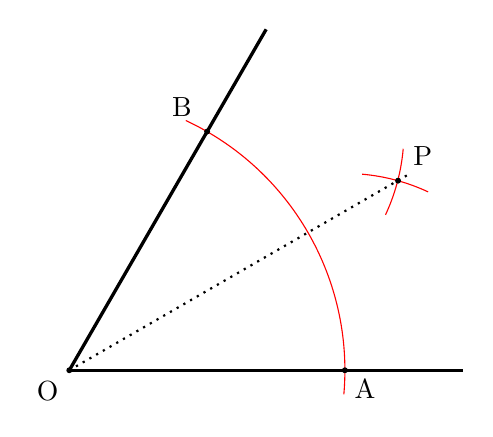
\begin{tikzpicture}
        \coordinate (O) at (0, 0);
        \coordinate (A) at (3.5, 0);
        \coordinate (B) at (1.75, 3.031);
        \coordinate (P) at (4.175, 2.408);

        \draw [-,very thick] node[below left] {\(\rm{O}\)} (O) -- (5, 0);
        \draw [-,very thick] (O) -- (2.5, 4.33);

        \draw[red] ([shift=(-5:3.5)] O) arc (-5:65:3.5);
        \draw[red] ([shift=(65:2.5)] A) arc (65:85:2.5);
        \draw[red] ([shift=(-25:2.5)] B) arc (-25:-5:2.5);
        \draw[dotted, thick] (O) -- (30:5);

        \filldraw[fill=black] (O) circle (0.03);
        \filldraw[fill=black] (A) circle (0.03) node[below right] {\(\rm{A}\)};
        \filldraw[fill=black] (B) circle (0.03) node[above left=2] {\(\rm{B}\)};
        \filldraw[fill=black] (P) circle (0.03) node[above right=2] {\(\rm{P}\)};
    \end{tikzpicture}
    \vspace*{-50px}
\end{wrapfigure}

다음은 각의 이등분선 \(\linesegment{OP}\)를 작도하는 방법이다.
\begin{enumerate}
    \item 컴퍼스를 벌려 \(\rm{O}\)를 중심으로 원의 일부(호)를 그린다.
    \item 그린 호와 각의 각 변의 교점을 각각 \(\rm{A}, \rm{B}\)라 하자.
    \item \(\rm{A}, \rm{B}\)를 중심으로 하는 호를 각각 그린다.
    \item 두 호의 교점을 \(\rm{P}\)라 하고, 자로 \(\linesegment{OP}\)를 그린다.
\end{enumerate}
위와 같이 작도한 \(\linesegment{OP}\)가 \(\angle \rm{AOB}\)의 이등분선임을 보여라.

\pagebreak

\section{귀류법}

때로는 주어진 명제를 직접 증명하기 어려운 경우가 있다. 예를 들어, \(\sqrt{2}\)가 무리수(순환하지 않는 무한소수)임을 보이려고 한다. 우선 무한소수인지 확인하려면 \(\sqrt{2}\)의 정확한 값을 열심히 계산해서 소수점 아래 어디선가 계산이 끝나는지 알아야 한다.

소수점 아래 1조 자리까지 계산했다고 치자. 아직 계산이 안 끝났지만, 계속 하다보면 끝날지도 모르므로 더 해보는 수밖에 없다. 100조 자리까지 계산했는데, 아직도 안 끝났다.\footnote{1조 자리까지 계산해도 무한히 많이 남았고, 100조 자리까지 계산해도 무한히 많이 남아있다. 남은 자리수가 비슷하니 왠지 계산을 별로 안 한 것 같다?} 그래도 더 해보는 수밖에 없는데, 이와 같은 방식은 매우 비효율적이다. 마찬가지로 순환마디가 존재하는지 확인하는 것도 직접 증명하려면 순환마디를 찾을 때까지 직접 계산하는 수밖에 없다.

이와 같은 경우 수학에서는 \textbf{귀류법}을 사용한다. 귀류법은 \textbf{증명하려는 명제의 결론을 부정한 후, 가정이나 잘 알려진 사실에 모순이 됨을 보이는 방법}이다. 만약 결론을 부정했을 때 오류를 얻는다면, 부정했던 결론이 오류의 원인이므로 원래 결론이 참이라고 주장하는 방식이다.

위 \(\sqrt{2}\)에 대한 예시의 경우, 결론을 부정하여 \(\sqrt{2}\)가 유리수라고 가정해보는 것이다. 만약 \(\sqrt{2}\)가 유리수라면, 수학적 사실이나 가정과 같이 우리가 참이라고 이미 받아들인 내용에 위배됨을 알 수 있다. 이와 같은 오류가 발생한 이유는 애초에 \(\sqrt{2}\)가 유리수라고 잘못 생각했기 때문이다. 따라서 \(\sqrt{2}\)는 무리수일 수밖에 없다고 결론 내린다.

\ex. 자연수는 무한함을 보여라.

\vspace*{80px}

\ex. 소수는 무한함을 보여라.

\vspace*{80px}

\ex. 유리수와 무리수의 합은 무리수임을 보여라.

\newpage

\section{수학적 귀납법}

자연수나 정수에 대한 명제를 증명하는 경우 \textbf{수학적 귀납법}을 사용할 수 있다.

\thm. (수학적 귀납법의 원리) 자연수에 대한 명제 \(p(n)\)에 대하여, 다음이 성립한다고 하자.
\begin{enumerate}
    \item \(p(1)\)이 참이다.
    \item 모든 자연수 \(n\)에 대하여 \(p(n)\)이 참일 때, \(p(n+1)\)이 참이다.
\end{enumerate}
그러면 모든 자연수 \(n\)에 대하여 \(p(n)\)이 참이다.

\pf 조건 (2)가 모든 \(n\)에 대하여 성립하므로 \(n = 1, 2, \dots\) 에 대해 적어보면
\[
    p(1) \ra p(2), \quad p(2) \ra p(3), \quad p(3) \ra p(4), \quad \dots
\]
이다. 그런데 \(p(1)\)이 참이므로 [명제 사용하기] 규칙에 의해 \(p(2)\)가 참이다. 같은 이유로 \(p(3)\)도 참이고, 같은 방식으로 계속 진행할 수 있다. 따라서 모든 자연수 \(n\)에 대하여 \(p(n)\)이 참이다. \qed

\textbf{수학적 귀납법의 핵심은 (2)번 조건에 있다.} \(p(1)\)이 참임을 보이는 것은 \(n = 1\) 로 두고 대입하여 직접 확인할 수 있기 때문에 어렵지 않은 반면, \(p(n)\)을 가정한 뒤 이로부터 \(p(n+1)\)이 참임을 끌어내는 과정은 자명하지 않기 때문이다.

이 과정을 생각해내기 위해서는 마찬가지로 \textbf{주어진 것과 구하는 것을 바탕으로 생각}하는 연습을 해야한다. (2)번 조건에서 주어진 것은 \(p(n)\)이고 구하는 것은 \(p(n+1)\)이다. \(p(n)\)과 \(p(n+1)\)의 차이 등을 분석하는 방법 등을 통해 이 둘을 어떻게 논리적으로 연결할 수 있을지 고민해야 한다.

\ex. 모든 자연수 \(n\)에 대하여 \(n(n+1)\)이 짝수임을 보여라.

\vspace*{100px}

\ex. 모든 자연수 \(n\)에 대하여 \(1 + 2 + \cdots + n = \dfrac{n(n+1)}{2}\) 임을 보여라.

\pagebreak

\section{반례 찾기}

수학에서 어떤 명제가 거짓임을 보이는 경우에는 적절한 반례를 찾으면 된다. 명제 \(p \ra q\) 가 참이라는 것은 \(p\)를 만족하는 모든 대상이 \(q\)를 만족한다는 의미인데, 만약 명제가 거짓이면 \textbf{\(p\)를 만족하는 모든 대상 중 \(q\)를 만족하지 않는 경우}가 존재한다는 뜻이다. 이런 경우가 바로 반례가 되므로, 반례를 찾을 때는 \textbf{\(p\)이면서 \(q\)가 아닌 대상}을 찾아야 한다.

\bigskip

다음 명제들에 대하여 참이면 증명하고, 거짓이면 반례를 들어라.

\ex. 정수 \(x, y\)에 대하여 \(x + y > 0\) 이면 \(x > 0\) 이다.

\vspace*{120px}

\ex. 두 정수가 아닌 유리수의 곱은 정수가 아닌 유리수이다.

\vspace*{120px}

\ex. 삼각형의 세 내각 중 적어도 하나는 \(60^\circ\)보다 크다.

\pagebreak
